\chapter{Архитектура}
\section{Классическая архитектура Android приложения}
Классическое приложение под Android состоит из разных компонентов, которые, как правило, указываются в специальном файле\textemdash\space Android Manifest.

\subsection*{Примеры компонентов:}
\begin{description}
	\item[Activity] Активность. Это ``фундаментальный'' компонент приложения, содержащий одну логическую единицу функциональности. Может содержать инструкции для отображения визуального пользовательского интерфейса и их макетов, управления потоком данных. Позволяет реализовывать парадигму ``Одно действие \textemdash\space один экран \textemdash\space одна активность''.
	\item[Fragment] Фрагмент. Представляет из себя переиспользуемую часть приложения, как правило отвечает за макет части визуального пользовательского интерфейса и связанную с ним логику.
	\item[Service] Сервис. Является механизмом выполнения постоянных, периодических или достаточно длительных действий в фоне. Запускается в общем потоке приложения. Бывает нескольких видов: активный, фоновый и привязанный.
	\item[Broadcast receiver] Получатель широковещательных сообщений. Предназначен для подписки на широковещательные сообщения от разных компонентов ОС и других приложений. Представляет из себя некоторую реализацию паттерна проектирования Listener.
\end{description}

Основной принцип проектирования приложений на Android \textemdash\space принцип разделённой ответственности: классы, связанные с отображением пользовательского интерфейса, содержат исключительно логику отображения этого интерфейса и взаимодействия с системой. Все остальное вынесено в другие функциональные блоки.

Данные обрабатываются в отдельных функциональных блоках, с учетом архитектуры MVP \textemdash\space в приложении есть три условных слоя, каждый из которых отвечает за свою часть работы приложения, их схема приведена на Рисунке \ref{fig:arch_uil_dol_dal}.

\begin{figure}[H]
	\centering
	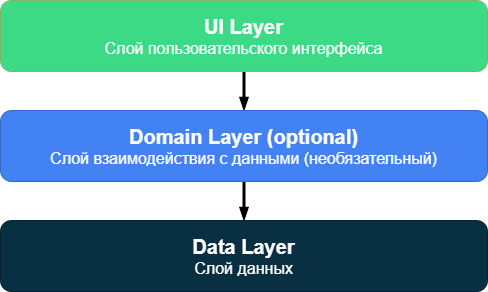
\includegraphics[width=\textwidth]{flesh/arch/uil-dol-dal.png}
	\caption{\label{fig:arch_uil_dol_dal}Схема архитектуры MVP}
\end{figure}

\subsection*{Обзор слоёв:}
\begin{description}
	\item[Слой пользовательского интерфейса] Этот слой иначе называют презентационным слоем. Его назначение – отображать данные приложения в том или ином виде на экране устройства. При изменении данных, взаимодействии с пользователем или поступлении внешнего ввода интерфейс должен соответствующим образом реагировать и отражать изменения.
	\item[Слой данных] Слой данных приложения содержит в себе «бизнес-логику». Бизнес-логика – это то, в чем есть суть приложения. Это правила, указывающие, как приложение создает, сохраняет и изменяет данные.
	Слой данных состоит из репозиториев, каждый из которых может содержать неотрицательное количество источников данных. Репозиторий создается на каждый отдельный тип данных, обрабатываемый в приложении.
	\item[Слой взаимодействия с данными] Иначе – слой доменов. Является опциональным слоем, расположен между презентационным слоем и слоем данных.
	Обычно представляет собой инкапсуляцию бизнес-логики, если она переиспользуется разными ViewModel объектами или если она достаточно объемная и сложная.
\end{description}

В минимально рабочем прототипе результирующего приложения также используется эта схема классической архитектуры.
Поскольку приложение работает с данными геолокации, в коде создан класс LocationEntity, отвечающий за единичную запись о геолокации устройства в конкретный момент времени. 
Он связан с объектами репозитория данных и доступа к данным. 
Эти объекты представляют собой слой данных в приложении.

Как такового слоя доменов в приложении нет, потому далее имеет смысл описать презентационный слой.

В приложении слой пользовательского интерфейса представлен следующими объектами:
\begin{description}
	\item[LocationUpdateViewModel] объект типа ViewModel, связывающий изменения в данных с изменениями в макете и его элементах;
	\item[LocationUpdateFragment] компонент типа Fragment, описывающий макет с отображаемым на экране содержимым и связанную с ним логику.
\end{description}

Таким образом с помощью применения стандартных компонентов и подходов к архитектуре реализуется корректный процесс работы с данными и интерфейсом в приложении под Android. 


\section{Компоненты бизнес-логики приложения}
\subsection{Сервисы}
Для управления ходом игры были созданы следующие сервисы:
\begin{description}
	\item[ScenarioService] Сервис, управляющий запуском и остановкой игровой сессии.
	\item[LocationService] Сервис, управляющий запуском и остановкой отслеживания геолокации в реальном времени.
	\item[HealthProtectionService] Сервис, обеспечивающий защиту здоровья игрока.
\end{description}
\smallskip
Дальше представлено более развёрнутое описание каждого из них.

\subsubsection*{ScenarioService}
Так как ScenarioService обеспечивает работу игровой сессии для него была включена настройка работы в фоне. Также этот сервис отвечает за запуск и остановку других игровых сервисов. 

ScenarioService не содержит в себе прямых методов запуска и остановки, которые можно было бы вызвать из активности, напротив, в нем используется встроенный механизм привязки сервисов Android: на событие привязки к активности и отвязки от активности происходит запуск с инициализацией и разрушение сервиса, соответственно.
\subsubsection*{LocationService}
Так как LocationService отвечает за бесперебойное получение данных о геолокации в реальном времени и должен уметь работать в фоне, он был реализован в виде стандартного сервиса Android. Так же как и ScenarioService, он не имеет методов для запуска и остановки, вызываемых из других компонент, при этом он запускается на присоединении к ScenarioService и имеет методы для включения или отключения работы в фоне.

\subsubsection*{HealthProtectionService}
Защита здоровья является важным компонентом с точки зрения заботы о пользователе. Представляет из себя подключаемый к ScenarioService сервис по аналогии с LocationService. 

При старте запускается таймер обратного отсчёта со следующими контрольными точками:
\begin{description}
	\item[За $N$ минут до истечения таймера] через голосовой интерфейс и вибрацию производится уведомление пользователя о необходимости завершить тренировку.
	\item[По истечении таймера] через голосовой интерфейс и вибрацию производится уведомление пользователя о принудительном завершении тренировки с фактическим её завершением.
\end{description}
\smallskip
При этом следует заметить, что таймер будет срабатывать при активности игровой сессии. При ручном$\backslash$аварийном (не инициированном пользователем или компонентом защиты здоровья) завершении игровой сессии таймер сбрасывается и не срабатывает до следующего запуска игровой сессии, когда он будет инициализирован заново.

\subsection{Менеджеры}
Менеджер \textemdash\space служебный класс, реализующий паттерн проектирования Singleton, так что во время работы приложения существует всегда только один объект этого класса, содержащий обрабатываемые данные.

Такие объекты нужны для хранения некоторого состояния приложения и данных игровой сессии.

В приложении были созданы следующие менеджеры:
\begin{description}
	\item[GeofencingManager] Менеджер обработки точек интереса и доступа к ним.
	\item[ActionsManager] Менеджер, управляющий событиями (генерация, финализация) и доступом к ним.
	\item[ObstaclesManager] Менеджер, управляющий препятствиями (генерация, финализация) и доступом к ним.
	\item[ScenarioManager] Менеджер обработки и управления запущенным сценарием геймификации.
	\item[SoundManager] Менеджер воспроизведения аудиконтента.
	\item[TTSManager] Менеджер воспроизведения звуковых нотификаций.
\end{description}
\smallskip
Далее представлено более подробное описание каждого из них.

\subsubsection*{GeofencingManager}
\label{subsubsec:geofencing_manager}
Объект данного класса хранит в себе активные во время игровой сессии точки интереса на карте и содержит методы управления ими:
\begin{description}
	\item[getActiveEntry] возвращает активную точку интереса, по которой ведется отслеживание в данный момент;
	\item[storeGeofence] добавляет точку интереса в очередь на ожидание;
	\item[processNext] финализирует активную точку интереса, помечает следующую в очереди как актуальную;
	\item[reset] очищает очередь точек интереса, сбрасывает активную, отключает отслеживание.
\end{description}

\subsubsection*{ActionsManager}
Объект данного класса хранит в себе активные во время игровой сессии таймеры и объекты сюжетных действий, а так же содержит методы управления ими:
\begin{description}
	\item[processEventAction] метод инициализации события, вызывается из ScenarioManager при предобработке сценария. 
	\item[scheduleAction] метод сохранения и запуска таймеров события, вызывается из processEventAction.
	\item[clear] очищает сохраненные данные по событиям и сбрасывает активные таймеры.
\end{description}

\subsubsection*{ObstaclesManager}
Объект данного класса хранит в себе на время игровой сессии виртуальные препятствия, а так же содержит методы управления ими:
\begin{description}
	\item[setCurrent] метод задания активного препятствия и запуска таймеров.
	\item[finalize] метод финализации препятствия.
	\item[clear] метод для очистки состояния препятствий.
\end{description}

\subsubsection*{SoundManager}
Объект данного класса одновременно хранит в себе активные во время игровой сессии точки интереса на карте и содержит методы управления ими:
\begin{description}
	\item[playTrack] метод для проигрывания музыкального трека из вложенных в приложение ресурсов.
	\item[stop] метод для остановки трека.
	\item[clear] метод для очистки состояния проигрывателя.
\end{description}

\subsubsection*{TTSManager}
Объект данного класса одновременно хранит в себе активные во время игровой сессии точки интереса на карте и содержит методы управления ими:
\begin{description}
	\item[speak] метод для озвучки голосовых инструкций системой TTS.
	\item[stop] метод для остановки озвучки голосовой инструкции через TTS.
\end{description}

\subsubsection*{ScenarioManager}
Объект данного класса так же, как и ScenarioService, является своего рода оркестратором описанных выше менеджеров. 
Содержит следующие методы:
\begin{description}
	\item[initialize] метод инициализации и предобработки сценария в заданном формате.
	\item[initializeCurrentChapter] метод инициализации текущей главы в рамках сценария.
	\item[runScenario] метод для запуска игровой сессии по загруженному сценарию.
	\item[finishChapter] метод завершения главы загруженного сценария по завершении игровой сессии.
	\item[clear] метод для очистки состояния менеджера.
\end{description}

\subsection{Получатели широковещательных сообщений}